\chapter[Guia de Uso]{Guia de Uso}

Nesse capítulo é apresentado como utilizar o SVN, através da explicação das primeiras configurações e das principais funcionalidades.

\section{Passo a passo para o primeiro contato com a ferramenta}

Nessa seção são apresentadas as configurações e os passos iniciais para a criação de um repositório utilizando o SVN. Nessa seção serão tratados:

\begin{itemize}

\item Criação de um repositório:
  
  \subitem Estrutura inicial do repositório;
  \subitem Estrutura recomendada do repositório;
  \subitem Configuração de acesso a um repositório;

\item Disponibilização de um repositório;

\item Acesso a um repositório;

\item Cópias de trabalho;
    \subitem Operações principais;

\end{itemize}

\subsection{Criando um repositório}

Agora que o SVN já está instalado, de acordo com \citeonline{svn-book}, para criação de um repositório deve ser dado o seguinte comando:

\begin{centering}

\colorbox{PineGreen}{
\begin{minipage}{250px}
  \textbf{svnadmin create <nome do repositorio>}

\end{minipage}
}
\end{centering}

Para importar uma pasta para o repositório, de acordo com \citeonline{wiki-svn}, deve ser dado o seguinte comando:


\begin{centering}

\colorbox{PineGreen}{
\begin{minipage}{450px}
  \textbf{svn import /caminho/da/pasta/a/ser/copiada file:///caminho/do/repositorio}

\end{minipage}
}
\end{centering}

\subsubsection{O repositório}

De acordo com \citeonline{svn-book}, quando você cria um repositório no SVN ele contém a estrutura de pastas da Figura \ref{fig:estrutura}.

\begin{figure}[!htb]
\centering
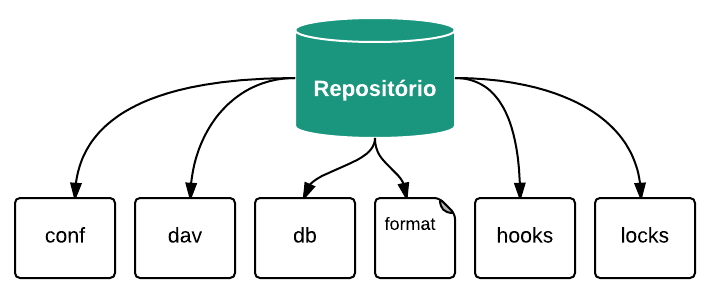
\includegraphics[scale=1]{figuras/repositorio.png}
\caption{Estrutura do repositório. Baseado em \cite{svn-book}}
\label{fig:estrutura}
\end{figure}

\pagebreak

\begin{itemize}

\item conf: Pasta que contém arquivos de configuração do repositório.

\item dav: Pasta que contém arquivos utilizados pelo mod\_dav\_svn.

\item db: Pasta que armazena os dados versionados.

\item format: Arquivo que indica o número da versão do repositório.

\item hooks: Pasta que contém modelos de scripts

\item locks: Pasta para arquivos bloqueados, é utilizado no rastreamento dos acessos ao repositório.

\end{itemize}


O repositório pode ser configurado com a estrutura de pastas que o usuário desejar, todavia existe um padrão recomendado que pode ser visto na Figura 
\ref{fig:estrutura_repo}.

\begin{figure}[!htb]
\centering
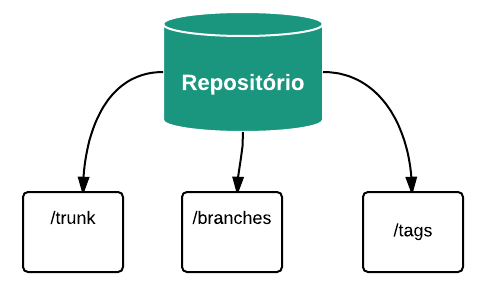
\includegraphics[scale=1]{figuras/estrutura_repo.png}
\caption{Estrutura recomendada do repositório. Baseado em \cite{svn-book}}
\label{fig:estrutura_repo}
\end{figure}

\begin{itemize}
  \item trunk: Pasta principal que contém os arquivos do repositório, é onde fica o projeto testado e sem erros. \cite{wiki-svn}

  \item branches: Pasta utilizada para guardar os arquivos do repositório, "onde você poderá usar para trabalhar em uma nova feature e depois fazer um merge dela com o mainline trunk". \cite{wiki-svn};

  \item tags: Pasta que armazena "snapshots da data do Release de uma dada versão". \cite{wiki-svn}
\end{itemize}

Para criar essa estrutura deve ser dado o comando a seguir para cada uma das pastas: \cite{wiki-svn}

\begin{centering}

\colorbox{PineGreen}{
\begin{minipage}{280px}
  \textbf{svn mkdir file:///caminho/do/repositorio/pasta}
\end{minipage}
}

\end{centering}

\subsubsection{Configurando o acesso ao repositório}
\label{secao_acesso}
Para configurar o controle de acesso ao repositório devem ser editados os arquivos: \cite{wiki-svn}

\begin{centering}
\colorbox{PineGreen}{
\begin{minipage}{250px}
  \textbf{caminho/do/repositorio/conf/svnserve.conf}
  \textbf{caminho/do/repositorio/conf/passwd}
\end{minipage}
}
\end{centering}

No arquivo \textit{svnserve.conf} deve ser descomentada a linha \textbf{password-db = passwd} e no arquivo \textit{svnserve.conf}
deve ser escrito o nome do usuário e a senha da seguinte forma: \textbf{usuário = senha}. \cite{wiki-svn}

\begin{centering}
Exemplo:

\colorbox{PineGreen}{
\begin{minipage}{100px}

  \textbf{usuario1 = 12345}
\end{minipage}
}
\end{centering}

\subsection{Disponibilizando um repositório}

Um repositório pode ser mantido apenas localmente e seu acesso torna-se restrito à máquina a qual ele foi criado. Mas isso não é muito vantajoso, dessa forma um repositório deve ser disponibilizado em um servidor para que as pessoas possam acessá-lo de qualquer lugar. As opções de servidor podem ser vistas no anexo \ref{servidores}. 

\subsection{Acessando um repositório}

  Os repositórios criados para controle de versão com o SVN são acessados através de URLs, seguindo os seguintes padrões: \cite{svn-book}

\begin{centering}

\textbf{Para o servidor:} É especificado o nome do servidor e a porta.

\colorbox{PineGreen}{
\begin{minipage}{220px}
  \textbf{http://svn.example.com:9834/repos}
\end{minipage}
}

\textbf{Para repositórios locais:} a URL ganha o prefixo \textit{file:}. Podem ser escritos com o nome do servidor, ou sem. E de acordo com \citeonline{wiki-svn}, para acessar repositórios locais deve apenas digitar o comando \textbf{svn co url\_definida}.
\end{centering}

\begin{multicols}{2} 


\flushright{O nome do servidor como \textit{localhost}:

\colorbox{PineGreen}{
\begin{minipage}{210px}
  \textbf{file://localhost/caminho/repositorio}
\end{minipage}
}
}

Ou sem especificação do servidor:

\colorbox{PineGreen}{
\begin{minipage}{200px}
\flushleft{ 
  \textbf{file:///caminho/repositorio}
}
\end{minipage}
}

\end{multicols}

As possíveis URLs de acesso podem ser vistas na Tabela \ref{tab:urls}.

\begin{table}[!h]
\centering
\caption{URLs de acesso ao repositório. Fonte: \cite{svn-book}}
\label{tab:urls}
\begin{tabular}{|l|l|}
\hline
\rowcolor[HTML]{01796F} 
{\color[HTML]{000000} \textbf{Esquema}} & {\color[HTML]{000000} \textbf{Método de Acesso}}                             \\ \hline
file:///                                & acesso direto ao repositório (em um disco local).                            \\ \hline
http://                                 & acesso via protocolo WebDAV em um servidor Apache especialmente configurado. \\ \hline
https://                                & mesmo que http://, mas com encriptação SSL.                                  \\ \hline
svn://                                  & acesso via protocolo próprio em um servidor svnserve.                        \\ \hline
svn+ssh://                              & mesmo que svn://, mas através de um túnel SSH.                               \\ \hline
\end{tabular}
\end{table}



\subsection{Cópias de trabalho}
  
O SVN trabalha com cópias de trabalho. Uma cópia de trabalho consiste na mesma estrutura do repositório para uso privado. Ou seja, é a cópia local do repositório que pode ser editada pelo usuário. 

Para criar uma cópia de trabalho deve ser digitado o seguinte comando: \citeonline{svn-book}


\begin{centering}
\colorbox{PineGreen}{
\begin{minipage}{320px}
  \textbf{svn checkout http://svn.example.com:9834/repositorio}
\end{minipage}
}

\end{centering}

\subsubsection{Como funciona a relação entre o repositório e a cópia de trabalho?}

\begin{figure}[!htb]
\centering
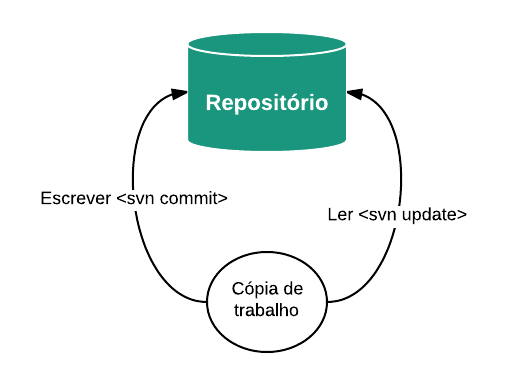
\includegraphics[scale=1]{figuras/repositorio_copia.png}
\caption{Comunicação entre cópia de trabalho e repositório. Baseado em \cite{svn-book}}
\end{figure}


Para que os outros membros do projeto tenham acesso ao que foi produzido na cópia de trabalho, o SVN permite que o usuário escreva no repositório as alterações feitas
e para ter acesso às atualizações feitas por outros membros, é permitido ao usuário ler o repositório. \cite{svn-book}

\begin{multicols}{2} 


\flushright{Para escrever}:{

\colorbox{PineGreen}{
\begin{minipage}{210px}
  \textbf{svn commit <nome do arquivo modificado> -m <"mensagem\">}
\end{minipage}
}
}

Para ler:

\colorbox{PineGreen}{
\begin{minipage}{100px}
\flushleft{ 
  \textbf{svn update}
}
\end{minipage}
}

\end{multicols}

\section{Passo a passo para o uso das principais funcionalidades da ferramenta}

Para ver os arquivos modificados o comando é: "svn status"

Para mostrar as diferenças m um arquivo "svn diff"

Para criar uma cópia de trabalho o comando é "svn checkout"

Para ver as revisões criadas o comando é: "svn status --verbose"

Para mostrar o histórico de mudanças o comando é "svn log"

Para desfazer as alterações em um arquivo: "svn revert <arquivo>"

Para criar uma branch, deve ser ser feita uma cópia da pasta trunk para a pasta de branchs com o seguinte comando:

"svn copy <caminho da pasta original> \ <caminho da pasta de destino, essa pasta deve possuir o nome da branch> -m "mensagem\">"

\section{Verificação das funcionalidades descritas a seguir em forma de pergunta:}

\begin{itemize}
  \item A ferramenta provê mecanismo de backup dos itens controlados pela ferramenta?

    Sim. O SVN provê um comando que possibilita a realização de um backup do repositório, caso algo dê errado. O comando é:
    "svnadmin hotcopy <caminho do repositorio> <caminho de backup>"

  \item A ferramenta provê algum mecanismo de controle de acesso?
    Sim. No arquivo "svnserve.conf" são descritos os níveis de acesso para usuários autenticados e não autenticados

  \item A ferramenta controla arquivos de diversos formatos, seja código, executáveis, documentação e diagramas?
    Sim. O SVN controla versão de todos os documentos colocados no repositório.

  \item A ferramenta registra versões dos itens de configuração?
    Sim. Cada alteração feita é registrada em um número de revisão. É possível visualizar um histórico de alterações com as seguintes informações:

    \subitem Nome do autor da alteração
    \subitem Data e hora
    \subitem Mensagem que descreve a alteração

  \item É possível visualizar as diferenças entre as versões incluindo a razão para estas 
  diferenças?

      O SVN permite a visualização das diferenças entre as versões, mas não apresenta a razão das diferenças.
  
  \item É possível identificar dependências entre artefatos, são elas: artefatos que pertencem a um mesmo item de configuração; itens de configuração de um componente; versão de itens de configuração de uma baseline; artefatos que são utilizados para construir um outro artefato  (por exemplo, um código é usado para construir a funcionalidade de um outro código)?
  
  
  \item É possível selecionar itens de configuração compatível com a versão válida e consistente do
  produto?
  \item É possível fazer snapshots ou congelar o estado de um produto a qualquer momento?
  \item A ferramenta provê mecanismos que facilitem a análise do impacto de se fazer uma mudança?
  \item É possível recuperar o histórico de todas as mudanças realizadas no itens controlados pela
  ferramenta?
  \item É possível recuperar o log de todos os detalhes do trabalho realizado?
  \item A ferramenta provê mecanismos para registrar estatísticas?
  \item A ferramenta provê mecanismos para examinar estado dos itens?
  \item A ferramenta provê mecanismos para selecionar aspectos para os quais deseja-se gerar relatório
  de acompanhamento de estado de configuração e gerar tal relatório?
  \item A ferramenta adverte sobre acesso inadequado a qualquer item para evitar mudanças não justificadas
  ou conflitos de mudanças?
  \item A ferramenta provê meios para monitorar bugs (quem, como e quando o bug foi gerado)?
  \item A ferramenta provê meios que facilitem a propagação de mudanças de maneira controlada
  através de diferentes versões de itens?
  \item A ferramenta provê mecanismos para facilitar a comunicação entre os interessados nos itens de
  configuração controlados?
  \item A ferramenta provê mecanismos para resolução de conflitos quando for necessário fazer merge
  de mudanças?
\end{itemize}
